\section{Softwarearchitektur und Design}

\subsection{Grundlagen und Überblick}

\begin{concept}{Grundlagen und Überblick}
\begin{itemize}
    \item \textbf{Business Analyse:}
    \begin{itemize}
        \item Domänenmodell und Kontextdiagramm
        \item Requirements (funktional und nicht-funktional)
        \item Vision und Stakeholder
    \end{itemize}
    
    \item \textbf{Architektur:}
    \begin{itemize}
        \item Logische Struktur des Systems
        \item Technische Konzeption
        \item Qualitätsanforderungen
    \end{itemize}
    
    \item \textbf{Entwicklung:}
    \begin{itemize}
        \item Use Case / User Story Realisierung
        \item Design-Klassendiagramm (DCD)
        \item Implementierung und Tests
    \end{itemize}
\end{itemize}
Architektur und Design sind eng verzahnt und bauen aufeinander auf:
\begin{itemize}
    \item Architektur definiert das "große Ganze"
    \item Design spezifiziert die Details der Umsetzung
    \item Beides basiert auf Requirements und führt zur Implementation
\end{itemize}
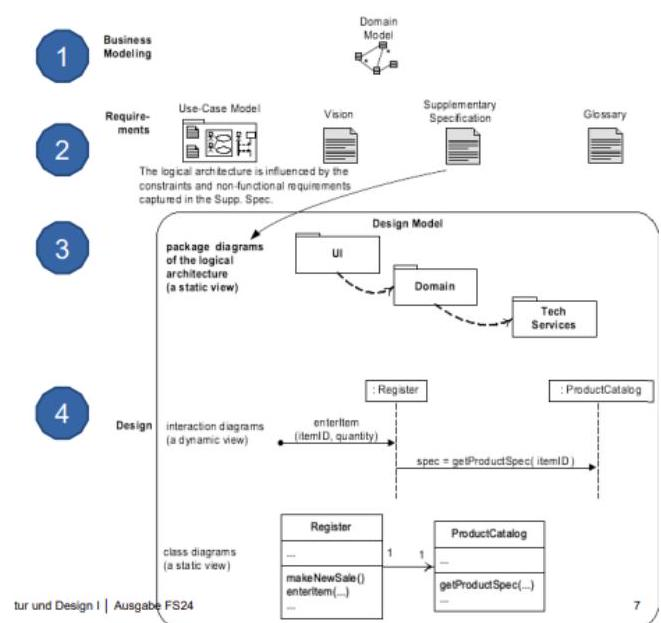
\includegraphics[width=\linewidth]{images/2024_12_29_0d1d7b5551ea1b4b41bdg-07(2)}
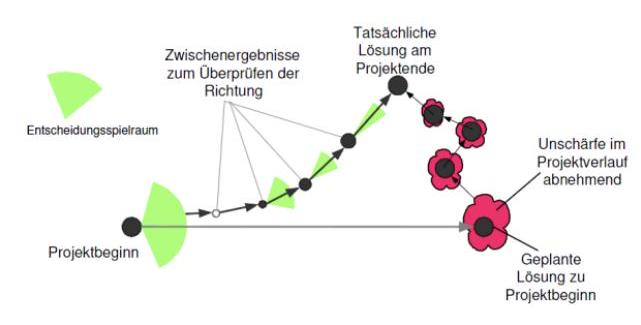
\includegraphics[width=\linewidth]{images/2024_12_29_0d1d7b5551ea1b4b41bdg-08(1)}
\end{concept}

\begin{definition}{Softwarearchitektur}
Die Architektur eines Softwaresystems definiert:

\begin{itemize}
    \item \textbf{Grundlegende Entscheidungen:}
    \begin{itemize}
        \item Programmiersprachen und Plattformen
        \item Aufteilung in Teilsysteme und Komponenten
        \item Schnittstellen zwischen Komponenten
    \end{itemize}
    
    \item \textbf{Strukturelle Aspekte:}
    \begin{itemize}
        \item Verantwortlichkeiten der Teilsysteme
        \item Abhängigkeiten zwischen Komponenten
        \item Einsatz von Basis-Technologien/Frameworks
    \end{itemize}
    
    \item \textbf{Qualitätsaspekte:}
    \begin{itemize}
        \item Erfüllung nicht-funktionaler Anforderungen
        \item Maßnahmen für Performance, Skalierbarkeit etc.
        \item Fehlertoleranz und Ausfallsicherheit
    \end{itemize}
\end{itemize}
\end{definition}

\begin{concept}{Architekturanalyse}\\
erfolgt iterativ mit den Anforderungen (Twin Peaks Model):

\begin{itemize}
    \item \textbf{Anforderungsanalyse:}
    \begin{itemize}
        \item Analyse funktionaler und nicht-funktionaler Anforderungen
        \item Prüfung der Qualität und Stabilität der Anforderungen
        \item Identifikation von Lücken und impliziten Anforderungen
    \end{itemize}
    
    \item \textbf{Architekturentscheidungen:}
    \begin{itemize}
        \item Abstimmung mit Stakeholdern
        \item Berücksichtigung von Randbedingungen
        \item Vorausschauende Planung für zukünftige Änderungen
    \end{itemize}
\end{itemize}

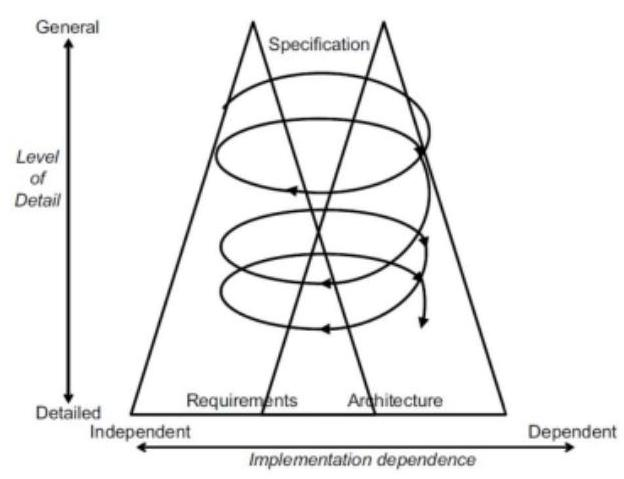
\includegraphics[width=0.9\linewidth]{images/2024_12_29_0d1d7b5551ea1b4b41bdg-08}
\end{concept}

\begin{theorem}{Qualitätsanforderungen}\\
\textbf{ISO 25010:}
\begin{itemize}
    \item Hierarchische Struktur für nicht-funktionale Anforderungen
    \item Definierte Hauptcharakteristiken und Subcharakteristiken
    \item Messbare Metriken für jede Anforderung
    \item Ermöglicht präzise Formulierung und Verifikation
\end{itemize}

\textbf{FURPS+:}
\begin{itemize}
    \item \textbf{F}unctionality (Funktionalität)
    \item \textbf{U}sability (Benutzerfreundlichkeit)
    \item \textbf{R}eliability (Zuverlässigkeit)
    \item \textbf{P}erformance (Leistung)
    \item \textbf{S}upportability (Wartbarkeit)
    \item \textbf{+}: Implementation, Interface, Operations, Packaging, Legal
\end{itemize}
\end{theorem}

\columnbreak

\subsection{Architektur-Design}

\begin{concept}{Modulkonzept}\\
Ein Modul (Baustein, Komponente) wird bewertet nach:
\begin{itemize}
    \item \textbf{Kohäsion:} Innerer Zusammenhang
    \item \textbf{Kopplung:} Externe Abhängigkeiten
\end{itemize}

\textbf{Eigenschaften:}
\begin{itemize}
    \item Autarkes Teilsystem
    \item Minimale externe Schnittstellen
    \item Enthält alle benötigten Funktionen/Daten
    \item Verschiedene Formen: Paket, Library, Service
\end{itemize}
\end{concept}

\begin{definition}{Schnittstellen}\\
Module kommunizieren über definierte Schnittstellen:

\begin{itemize}
    \item \textbf{Exportierte Schnittstellen:}
    \begin{itemize}
        \item Definieren angebotene Funktionalität
        \item Vertraglich garantierte Leistungen
        \item Einzige nach außen sichtbare Information
    \end{itemize}
    
    \item \textbf{Importierte Schnittstellen:}
    \begin{itemize}
        \item Von anderen Modulen benötigte Funktionalität
        \item Definieren Abhängigkeiten
        \item Basis für Kopplung
        \item Sollten minimiert werden (Low Coupling)
    \end{itemize}
\end{itemize}
\end{definition}

\begin{concept}{Architektursichten (4+1 View Model)}\\
Verschiedene Perspektiven auf die Architektur:

\begin{itemize}
    \item \textbf{Logical View:} End-User, Functionality
    \begin{itemize}
        \item Funktionalität des Systems
        \item Schichten, Subsysteme, Pakete
        \item Klassen und Schnittstellen
    \end{itemize}
    
    \item \textbf{Process View:} Integrators, Performance, Scalability
    \begin{itemize}
        \item Laufzeitverhalten
        \item Prozesse und Threads
        \item Performance und Skalierung
    \end{itemize}

    \item \textbf{Development View:} Programmers, Software Management
    \begin{itemize}
        \item Implementierungsstruktur
        \item Quellcode-Organisation
        \item Build und Deployment
    \end{itemize}
    
    \item \textbf{Physical View:} System Engineers, Topology, Communications
    \begin{itemize}
        \item Hardware-Topologie
        \item Verteilung der Software
        \item Netzwerkkommunikation
    \end{itemize}
\end{itemize}

    
\textbf{+1: Scenarios:}
    \begin{itemize}
        \item Wichtige Use Cases
        \item Validierung der Architektur
        \item Integration der anderen Views
    \end{itemize}
%todo: better resolution image
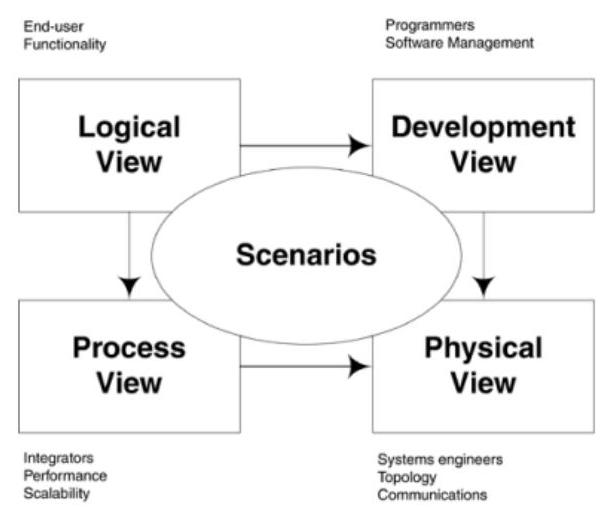
\includegraphics[width=0.9\linewidth]{images/2024_12_29_0d1d7b5551ea1b4b41bdg-09}
\end{concept}

\begin{concept}{Architekturprinzipien}
Grundlegende Prinzipien für gute Architektur:

\textbf{Separation of Concerns:}
\begin{itemize}
    \item Trennung von Verantwortlichkeiten
    \item Klare Modulgrenzen
    \item Reduzierte Komplexität
\end{itemize}

\textbf{Information Hiding:}
\begin{itemize}
    \item Kapselung von Implementierungsdetails
    \item Definierte Schnittstellen
    \item Änderbarkeit ohne Seiteneffekte
\end{itemize}

\textbf{Loose Coupling:}
\begin{itemize}
    \item Minimale Abhängigkeiten
    \item Austauschbarkeit
    \item Unabhängige Entwicklung
\end{itemize}
\end{concept}


\begin{corollary}{Qualitätskriterien und deren Umsetzung}\\
Strategien zur Erfüllung von Qualitätsanforderungen:

\textbf{Performance:}
\begin{itemize}
    \item Effiziente Ressourcennutzung (Resource Pooling, Caching)
    \item Optimierte Verarbeitung (Parallelisierung, Lazy Loading)
\end{itemize}

\textbf{Skalierbarkeit:}
\begin{itemize}
    \item Dynamische Anpassung (horizontale/vertikale Skalierung)
    \item Effiziente Lastverteilung (Load Balancing, Partitionierung)
\end{itemize}

\textbf{Wartbarkeit:}
\begin{itemize}
    \item Klare Strukturen (Separation of Concerns, Modularisierung)
    \item Verbesserte Codequalität (Information Hiding, Standardisierung)
\end{itemize}

\textbf{Zuverlässigkeit:}
\begin{itemize}
    \item Fehlerresistenz (Redundanz, Fehlertoleranz)
    \item Prävention und Wiederherstellung (Monitoring, Backup/Recovery)
\end{itemize}

\textbf{Verfügbarkeit:}
\begin{itemize}
    \item Ausfallschutz (Redundanz, Failover-Mechanismen)
    \item Überwachung/Stabilisierung (Health Monitoring, Circuit Breaker)
\end{itemize}

\textbf{Modularität:}
\begin{itemize}
    \item Gut definierte Grenzen (klare Modulgrenzen, hohe Kohäsion)
    \item Minimale Abhängigkeiten zwischen Modulen
\end{itemize}

\textbf{Testbarkeit:}
\begin{itemize}
    \item Einfachheit von Tests (Isolation, Mockbarkeit)
    \item Automatisierung und Skalierung von Tests
\end{itemize}

\textbf{Änderbarkeit:}
\begin{itemize}
    \item Anpassungsfähigkeit (Lokalisierung, Erweiterbarkeit)
    \item Sicherstellung der Kompatibilität (Backward Compatibility)
\end{itemize}

\textbf{Erweiterbarkeit:}
\begin{itemize}
    \item Flexible Architekturen (offene Schnittstellen, Plugin-Systeme)
    \item Serviceorientierung für modulare Erweiterungen
\end{itemize}
\end{corollary}

\subsection{Architekturprozess und Best Practices}
%todo: make easier to understand, remove redundant information, make more concise, add examples from Wissenssicherungen and missing information from the slides

\begin{formula}{Best Practices im Architekturentwurf}\\
\textbf{1. Analyse und Planung}
\begin{itemize}
    \item Anforderungen priorisieren
    \item Qualitätsziele definieren
    \item Constraints identifizieren
    \item Stakeholder einbinden
\end{itemize}

\textbf{2. Design-Prinzipien}
\begin{itemize}
    \item Separation of Concerns
    \item Single Responsibility
    \item Information Hiding
    \item Don't Repeat Yourself (DRY)
\end{itemize}

\textbf{3. Strukturierung}
\begin{itemize}
    \item Klare Schichtenarchitektur
    \item Definierte Schnittstellen
    \item Lose Kopplung
    \item Hohe Kohäsion
\end{itemize}

\textbf{4. Dokumentation}
\begin{itemize}
    \item Architekturentscheidungen
    \item Begründungen
    \item Alternativen
    \item Trade-offs
\end{itemize}
\end{formula}

\subsubsection{Gesamter Architekturprozess}

\begin{definition}{Architekturprozess-Komponenten}\\
\textbf{Architekturanalyse:}
\begin{itemize}
    \item Erster Schritt im Architekturprozess
    \item Analyse der funktionalen und nicht-funktionalen Anforderungen
    \item Identifikation von Qualitätszielen
    \item Parallel zur Anforderungserhebung (Twin Peaks)
\end{itemize}

\textbf{Architektur-Entscheidungen:}
\begin{itemize}
    \item Konkrete Beschlüsse basierend auf der Analyse
    \item Technologiewahl und Strukturierung
    \item Dokumentation und Begründung
    \item Einschließlich verworfener Alternativen
\end{itemize}

\textbf{Architektur-Entwurf:}
\begin{itemize}
    \item Praktischer Gestaltungsprozess
    \item Anwendung von Architekturmustern
    \item Umsetzung von Qualitätsanforderungen
    \item Erstellung konkreter Artefakte
\end{itemize}

\textbf{Architektur-Review:}
\begin{itemize}
    \item Systematische Überprüfung
    \item Meist durch externe Experten
    \item Prüfung der Anforderungserfüllung
    \item Identifikation von Schwachstellen
\end{itemize}

\textbf{Architektur-Evaluation:}
\begin{itemize}
    \item Bewertung anhand definierter Kriterien
    \item Quantitative und qualitative Analyse
    \item Szenario-basierte Prüfung
    \item Bewertung von Qualitätsattributen
\end{itemize}
\end{definition}

\begin{KR}{Gesamter Architekturprozess}\\
\textbf{1. Initiale Phase}
\begin{itemize}
    \item Architekturanalyse durchführen
    \item Grundlegende Entscheidungen treffen
    \item Ersten Entwurf erstellen
\end{itemize}

\textbf{2. Iterative Verfeinerung}
\begin{itemize}
    \item Review durchführen
    \item Evaluation vornehmen
    \item Anpassungen basierend auf Feedback
\end{itemize}

\textbf{3. Kontinuierliche Verbesserung}
\begin{itemize}
    \item Regelmäßige Reviews
    \item Neue Anforderungen einarbeiten
    \item Technische Schulden adressieren
\end{itemize}

\textbf{4. Dokumentation}
\begin{itemize}
    \item Entscheidungen festhalten
    \item Architektur dokumentieren
    \item Änderungen nachverfolgen
\end{itemize}

\textbf{5. Qualitätssicherung}
\begin{itemize}
    \item Architektur-Konformität prüfen
    \item Performance-Tests durchführen
    \item Sicherheitsaudits durchführen
\end{itemize}
\end{KR}

\begin{example2}{Gesamter Architekturprozess}\\
    %todo: add example
\end{example2}


\begin{KR}{Architekturanalyse}\\
\textbf{1. Anforderungen sammeln}
\begin{itemize}
    \item Funktionale Anforderungen gruppieren
    \item Nicht-funktionale Anforderungen identifizieren
    \item Randbedingungen dokumentieren
\end{itemize}

\textbf{2. Qualitätsziele definieren}
\begin{itemize}
    \item Messbare Kriterien festlegen
    \item Priorisierung vornehmen
    \item Trade-offs identifizieren
\end{itemize}

\textbf{3. Einflussfaktoren analysieren}
\begin{itemize}
    \item Technische Faktoren
    \item Organisatorische Faktoren
    \item Wirtschaftliche Faktoren
\end{itemize}
\end{KR}

\begin{example2}{Architekturanalyse}\\
    %todo: add example    
\end{example2}

\begin{KR}{Architektur-Entscheidungen}\\
\textbf{1. Alternativen identifizieren}
\begin{itemize}
    \item Mögliche Lösungen sammeln
    \item Vor- und Nachteile analysieren
    \item Machbarkeit prüfen
\end{itemize}

\textbf{2. Bewertungskriterien}
\begin{itemize}
    \item Erfüllung der Anforderungen
    \item Technische Umsetzbarkeit
    \item Kosten und Aufwand
\end{itemize}

\textbf{3. Entscheidung dokumentieren}
\begin{itemize}
    \item Begründung
    \item Konsequenzen
    \item Verworfene Alternativen
\end{itemize}
\end{KR}

\begin{corollary}{Architektur-Entscheidungen dokumentieren}\\
\textbf{1. Entscheidung festhalten}
\begin{itemize}
    \item Dokumentation der getroffenen Architekturentscheidungen
    \item Begründungen und Alternativen
    \item Auswirkungen und Konsequenzen
\end{itemize}

\textbf{2. Strukturierte Dokumentation}
\begin{itemize}
    \item Einheitliches Format für alle Entscheidungen
    \item Verwendung von Templates
    \item Nachvollziehbare Historie der Entscheidungen
\end{itemize}

\textbf{3. Kommunikation}
\begin{itemize}
    \item Regelmäßige Updates an Stakeholder
    \item Transparenz über getroffene Entscheidungen
    \item Einbindung des gesamten Teams
\end{itemize}

\textbf{4. Review und Anpassung}
\begin{itemize}
    \item Regelmäßige Überprüfung der Entscheidungen
    \item Anpassung bei geänderten Rahmenbedingungen
    \item Lessons Learned dokumentieren
\end{itemize}
\end{corollary}

\begin{example2}{Architektur-Entscheidungen}\\
    %todo: add example    
\end{example2}


\begin{KR}{Architekturentwurf}\\
\textbf{Schritte:}
\begin{enumerate}
    \item Anforderungen analysieren
    \item Architekturstil wählen
    \item Module identifizieren
    \item Schnittstellen definieren
    \item Mit Stakeholdern abstimmen
\end{enumerate}
\end{KR}

\begin{example2}{Architekturentwurf}\\
    %todo: add example
\end{example2}

\begin{KR}{Architektur-Review durchführen}\\
\textbf{Vorgehen:}
\begin{enumerate}
    \item \textbf{Vorbereitung}
    \begin{itemize}
        \item Architektur-Dokumentation zusammenstellen
        \item Review-Team zusammenstellen
        \item Checklisten vorbereiten
    \end{itemize}
    
    \item \textbf{Durchführung}
    \begin{itemize}
        \item Architektur vorstellen
        \item Anforderungen prüfen
        \item Entscheidungen hinterfragen
        \item Risiken identifizieren
    \end{itemize}
    
    \item \textbf{Nachbereitung}
    \begin{itemize}
        \item Findings dokumentieren
        \item Maßnahmen definieren
        \item Follow-up planen
    \end{itemize}
\end{enumerate}

\textbf{Prüfkriterien:}
\begin{itemize}
    \item Anforderungserfüllung
    \item Technische Machbarkeit
    \item Zukunftssicherheit
    \item Best Practices
\end{itemize}
\end{KR}

\begin{example2}{Architektur-Review}\\
    %todo: add example    
\end{example2}



\begin{KR}{Architektur-Evaluation}\\
Systematische Bewertung einer Softwarearchitektur:

\textbf{1. Qualitätsattribute identifizieren}
\begin{itemize}
    \item Performance
    \item Skalierbarkeit
    \item Wartbarkeit
    \item Sicherheit
\end{itemize}

\textbf{2. Szenarien entwickeln}
\begin{itemize}
    \item Normale Nutzung
    \item Grenzfälle
    \item Fehlerfälle
    \item Wartungsszenarien
\end{itemize}

\textbf{3. Architektur analysieren}
\begin{itemize}
    \item Strukturanalyse
    \item Verhaltensanalyse
    \item Trade-off Analyse
\end{itemize}

\textbf{4. Risiken identifizieren}
\begin{itemize}
    \item Technische Risiken
    \item Geschäftsrisiken
    \item Architekturrisiken
\end{itemize}
\end{KR}

\begin{example2}{Architektur-Evaluation}\\
    %todo: add example    
\end{example2}


\pagebreak


\subsection{Architekturmuster}

%todo: remove redundant information, make more concise, add definition of each pattern, add examples from Wissenssicherungen and missing information from the slides
%my proposal for the structure of this section is to first define the patterns and then give examples of each pattern (every pattern listed in Übersicht Architekturmuster should have an example)
%and obviously, if there is one missing from the slides add that too

\begin{concept}{Übersicht Architekturmuster}\\
Grundlegende Architekturmuster für Software-Systeme:

\begin{itemize}
    \item \textbf{Layered Pattern:} 
    \begin{itemize}
        \item Strukturierung in horizontale Schichten
        \item Klare Trennung der Verantwortlichkeiten
        \item Abhängigkeiten nur nach unten
    \end{itemize}
    
    \item \textbf{Client-Server Pattern:}
    \begin{itemize}
        \item Verteilung von Diensten
        \item Zentralisierte Ressourcen
        \item Mehrere Clients pro Server
    \end{itemize}
    
    \item \textbf{Master-Slave Pattern:}
    \begin{itemize}
        \item Verteilung von Aufgaben
        \item Zentrale Koordination
        \item Parallelverarbeitung
    \end{itemize}
    
    \item \textbf{Pipe-Filter Pattern:}
    \begin{itemize}
        \item Datenstromverarbeitung
        \item Verkettung von Operationen
        \item Wiederverwendbare Filter
    \end{itemize}
    
    \item \textbf{Broker Pattern:}
    \begin{itemize}
        \item Vermittlung zwischen Komponenten
        \item Entkopplung von Diensten
        \item Zentrale Koordination
    \end{itemize}
    
    \item \textbf{Event-Bus Pattern:}
    \begin{itemize}
        \item Asynchrone Kommunikation
        \item Publisher-Subscriber Modell
        \item Lose Kopplung
    \end{itemize}
\end{itemize}
\end{concept}

\begin{concept}{Clean Architecture}\\
Architektur-Prinzipien nach Robert C. Martin:

\textbf{Hauptprinzipien:}
\begin{itemize}
    \item Unabhängigkeit von Frameworks
    \item Unabhängigkeit von UI
    \item Unabhängigkeit von Datenbank
    \item Testbarkeit ohne externe Systeme
\end{itemize}

\textbf{Schichten (von innen nach außen):}
\begin{itemize}
    \item \textbf{Entities:} 
    \begin{itemize}
        \item Zentrale Geschäftsregeln
        \item Unternehmensweit gültig
        \item Höchste Stabilität
    \end{itemize}
    
    \item \textbf{Use Cases:}
    \begin{itemize}
        \item Anwendungsspezifische Geschäftsregeln
        \item Orchestrierung der Entities
        \item Anwendungslogik
    \end{itemize}
    
    \item \textbf{Interface Adapters:}
    \begin{itemize}
        \item Konvertierung von Daten
        \item Präsentation und Controller
        \item Gateway-Implementierungen
    \end{itemize}
    
    \item \textbf{Frameworks \& Drivers:}
    \begin{itemize}
        \item UI-Framework
        \item Datenbank
        \item Externe Schnittstellen
    \end{itemize}
\end{itemize}
\end{concept}

\begin{KR}{Clean Architecture}\\
Prinzipien nach Robert C. Martin:

\begin{itemize}
    \item \textbf{Unabhängigkeit von Frameworks}
    \begin{itemize}
        \item Framework als Tool, nicht als Einschränkung
        \item Geschäftslogik unabhängig von UI/DB
    \end{itemize}
    
    \item \textbf{Testbarkeit}
    \begin{itemize}
        \item Business Rules ohne externe Systeme testbar
        \item Keine DB/UI für Tests notwendig
    \end{itemize}
    
    \item \textbf{Unabhängigkeit von UI}
    \begin{itemize}
        \item UI austauschbar ohne Business Logic Änderung
        \item Web, Desktop, Mobile möglich
    \end{itemize}
    
    \item \textbf{Unabhängigkeit von Datenbank}
    \begin{itemize}
        \item DB-System austauschbar
        \item Business Rules unabhängig von Datenpersistenz
    \end{itemize}
\end{itemize}

\textbf{Schichten von außen nach innen:}
\begin{enumerate}
    \item Frameworks \& Drivers (UI, DB, External Interfaces)
    \item Interface Adapters (Controllers, Presenters)
    \item Application Business Rules (Use Cases)
    \item Enterprise Business Rules (Entities)
\end{enumerate}
\end{KR}

\begin{KR}{Clean Architecture}
Prinzipien nach Robert C. Martin:

\textbf{Hauptprinzipien:}
\begin{itemize}
    \item Unabhängigkeit von Frameworks
    \item Testbare Business Rules
    \item Unabhängigkeit von UI
    \item Unabhängigkeit von Datenbank
    \item Unabhängigkeit von externen Systemen
\end{itemize}

\textbf{Schichten (von innen nach außen):}
\begin{enumerate}
    \item Entities (Enterprise Business Rules)
    \item Use Cases (Application Business Rules)
    \item Interface Adapters (Controllers, Presenters)
    \item Frameworks \& Drivers (UI, DB, Devices)
\end{enumerate}

\textbf{Dependency Rule:}
Abhängigkeiten dürfen nur nach innen zeigen.
\end{KR}

\begin{concept}{Schichtenarchitektur (Layered Architecture)}\\
Strukturierung eines Systems in horizontale Schichten:

\textbf{Typische Schichten:}
\begin{itemize}
    \item Präsentationsschicht (UI)
    \item Anwendungsschicht (Application)
    \item Geschäftslogikschicht (Domain)
    \item Datenzugriffsschicht (Persistence)
\end{itemize}

\textbf{Regeln:}
\begin{itemize}
    \item Kommunikation nur mit angrenzenden Schichten
    \item Abhängigkeiten nur nach unten
    \item Jede Schicht kapselt ihre Implementierung
\end{itemize}
\end{concept}

\begin{concept}{Schichtenarchitektur (Layered Architecture)}\\
Organisation des Systems in hierarchische Schichten:

\textbf{Typische Schichten:}
\begin{itemize}
    \item Präsentationsschicht (UI)
    \item Anwendungsschicht (Application Logic)
    \item Geschäftslogikschicht (Domain Logic)
    \item Datenzugriffsschicht (Data Access)
\end{itemize}

\textbf{Prinzipien:}
\begin{itemize}
    \item Schichten kommunizieren nur mit direkten Nachbarn
    \item Abhängigkeiten nur nach unten
    \item Jede Schicht kapselt ihre Implementierung
    \item Höhere Schichten sind von unteren abhängig
\end{itemize}

\begin{lstlisting}[language=Java, style=basesmol]
// Praesentationsschicht
public class CustomerController {
    private CustomerService service;
    
    public CustomerDTO getCustomer(String id) {
        return service.findCustomer(id);
    }
}

// Anwendungsschicht
public class CustomerService {
    private CustomerRepository repository;
    
    public CustomerDTO findCustomer(String id) {
        Customer customer = repository.findById(id);
        return CustomerDTO.from(customer);
    }
}

// Geschaeftslogikschicht
public class Customer {
    private CustomerId id;
    private String name;
    
    public void updateName(String newName) {
        validateName(newName);
        this.name = newName;
    }
}

// Datenzugriffsschicht
public class CustomerRepository {
    public Customer findById(String id) {
        // Datenbankzugriff
    }
}
\end{lstlisting}
\end{concept}


\begin{example2}{Schichtenarchitektur Implementation}\\
\textbf{Beispiel einer typischen Schichtenstruktur:}

\begin{lstlisting}[language=Java, style=basesmol]
// Presentation Layer
public class CustomerController {
    private CustomerService service;
    
    public CustomerDTO getCustomer(String id) {
        Customer customer = service.findById(id);
        return CustomerDTO.from(customer);
    }
}

// Application Layer
public class CustomerService {
    private CustomerRepository repository;
    
    public Customer findById(String id) {
        validateId(id);
        return repository.findById(id)
            .orElseThrow(CustomerNotFoundException::new);
    }
}

// Domain Layer
public class Customer {
    private CustomerId id;
    private String name;
    private Address address;
    
    public void updateAddress(Address newAddress) {
        validateAddress(newAddress);
        this.address = newAddress;
    }
}

// Persistence Layer
public class CustomerRepository {
    private JpaRepository<Customer, CustomerId> jpaRepo;
    
    public Optional<Customer> findById(String id) {
        return jpaRepo.findById(new CustomerId(id));
    }
}
\end{lstlisting}
\end{example2}



\begin{concept}{Client-Server Architektur}\\
Verteilung von Funktionalitäten zwischen Client und Server:

\textbf{Charakteristiken:}
\begin{itemize}
    \item Klare Trennung von Zuständigkeiten
    \item Zentralisierte Ressourcenverwaltung
    \item Skalierbarkeit durch Server-Erweiterung
    \item Verschiedene Client-Typen möglich
\end{itemize}

\textbf{Varianten:}
\begin{itemize}
    \item Thin Client: Minimale Client-Logik
    \item Rich Client: Komplexe Client-Funktionalität
    \item Web Client: Browser-basiert
    \item Mobile Client: Für mobile Geräte optimiert
\end{itemize}
\end{concept}





\subsection{Objektorientiertes Design}

%todo: remove redundant information, make more concise, add examples from Wissenssicherungen and missing information from the slides
%here is my proposal for the structure of this section:
%- GRASP Prinzipien
%- Responsibility Driven Design
%- Design Patterns in der Architektur
%- Anti-Patterns

\subsubsection{Objektorientiertes Design}

\begin{concept}{GRASP Prinzipien}\\
General Responsibility Assignment Software Patterns - Grundlegende Prinzipien für die Zuweisung von Verantwortlichkeiten:

\textbf{Information Expert:}
\begin{itemize}
    \item Zuständigkeit basierend auf Information
    \item Klasse mit relevanten Daten übernimmt Aufgabe
    \item Fördert Kapselung und Kohäsion
\end{itemize}

\textbf{Creator:}
\begin{itemize}
    \item Verantwortung für Objekterstellung
    \item Basierend auf Beziehungen (enthält, aggregiert)
    \item Starke Verwendungsbeziehung
\end{itemize}

\textbf{Controller:}
\begin{itemize}
    \item Koordination von Systemoperationen
    \item Erste Anlaufstelle nach UI
    \item Fassade für Subsystem
\end{itemize}

\textbf{Low Coupling:}
\begin{itemize}
    \item Minimale Abhängigkeiten
    \item Erhöht Wiederverwendbarkeit
    \item Erleichtert Änderungen
\end{itemize}

\textbf{High Cohesion:}
\begin{itemize}
    \item Fokussierte Verantwortlichkeiten
    \item Zusammengehörige Funktionalität
    \item Wartbare Klassen
\end{itemize}
\end{concept}

\begin{concept}{Design nach GRASP}\\
General Responsibility Assignment Software Patterns:

\textbf{Grundprinzipien:}
\begin{itemize}
    \item \textbf{Information Expert:} Verantwortlichkeit dort, wo die Information liegt
    \item \textbf{Creator:} Objekterstellung durch eng verbundene Klassen
    \item \textbf{Controller:} Koordination von Systemoperationen
    \item \textbf{Low Coupling:} Minimale Abhängigkeiten zwischen Klassen
    \item \textbf{High Cohesion:} Starker innerer Zusammenhang in Klassen
\end{itemize}

\textbf{Erweiterte Prinzipien:}
\begin{itemize}
    \item \textbf{Polymorphism:} Typenabhängiges Verhalten durch Polymorphie
    \item \textbf{Pure Fabrication:} Hilfsklassen für besseres Design
    \item \textbf{Indirection:} Vermittler für lose Kopplung
    \item \textbf{Protected Variations:} Kapselung von Änderungen
\end{itemize}
\end{concept}

\begin{example2}{GRASP in der Praxis}\\
\begin{lstlisting}[language=Java, style=base]
// Information Expert: Order kennt seine Details
public class Order {
    private List<OrderLine> lines;
    
    public Money calculateTotal() {
        return lines.stream()
                   .map(OrderLine::getSubtotal)
                   .reduce(Money.ZERO, Money::add);
    }
}

// Controller: Koordiniert Use Case
public class OrderController {
    private OrderService service;
    
    public OrderResponse createOrder(OrderRequest request) {
        // Koordination der Verarbeitung
        Order order = service.createOrder(request);
        return OrderResponse.from(order);
    }
}

// Protected Variations: Abstraktion von Implementierung
public interface PaymentGateway {
    PaymentResult process(Money amount);
}

public class StripePaymentGateway implements PaymentGateway {
    public PaymentResult process(Money amount) {
        // Stripe-spezifische Implementierung
    }
}
\end{lstlisting}
\end{example2}

\begin{concept}{Responsibility Driven Design}\\
Designansatz basierend auf Verantwortlichkeiten und Kollaborationen:

\textbf{Verantwortlichkeiten:}
\begin{itemize}
    \item \textbf{Doing:}
    \begin{itemize}
        \item Aktionen ausführen
        \item Berechnungen durchführen
        \item Andere Objekte steuern
    \end{itemize}
    
    \item \textbf{Knowing:}
    \begin{itemize}
        \item Eigene Daten kennen
        \item Verwandte Objekte kennen
        \item Berechnete Informationen
    \end{itemize}
\end{itemize}

\textbf{Kollaborationen:}
\begin{itemize}
    \item Klare Rollen definieren
    \item Aufgaben verteilen
    \item Interfaces abstimmen
\end{itemize}
\end{concept}

\begin{concept}{Design Pattern Kategorien}\\
Bewährte Lösungsmuster für wiederkehrende Designprobleme:

\textbf{Erzeugungsmuster (Creational):}
\begin{itemize}
    \item Abstract Factory: Familien verwandter Objekte
    \item Factory Method: Objekterzeugung in Subklassen
    \item Singleton: Genau eine Instanz
    \item Builder: Komplexe Objektkonstruktion
    \item Prototype: Klonen existierender Objekte
\end{itemize}

\textbf{Strukturmuster (Structural):}
\begin{itemize}
    \item Adapter: Schnittstellen anpassen
    \item Bridge: Implementation von Abstraktion trennen
    \item Composite: Teil-Ganzes Hierarchien
    \item Decorator: Dynamische Funktionserweiterung
    \item Facade: Vereinfachte Schnittstelle
    \item Proxy: Kontrollierter Zugriff
\end{itemize}

\textbf{Verhaltensmuster (Behavioral):}
\begin{itemize}
    \item Command: Anfrage als Objekt
    \item Observer: Ereignisbenachrichtigung
    \item Strategy: Austauschbare Algorithmen
    \item Template Method: Algorithmus-Skelett
    \item State: Zustandsabhängiges Verhalten
    \item Visitor: Operation zu Objektstruktur hinzufügen
\end{itemize}
\end{concept}

\subsubsection{Design Patterns in der Architektur} %id this the right place for this?

\begin{concept}{Model-View-Controller (MVC)}\\
Trennt Anwendung in drei Hauptkomponenten:
\begin{itemize}
    \item \textbf{Model:} Geschäftslogik und Daten
    \item \textbf{View:} Darstellung der Daten
    \item \textbf{Controller:} Steuerung und Koordination
\end{itemize}

\begin{lstlisting}[language=Java, style=basesmol]
// Model
public class CustomerModel {
    private String name;
    private List<Order> orders;
    
    public void addOrder(Order order) {
        orders.add(order);
        notifyViews();
    }
}

// View
public class CustomerView {
    private CustomerModel model;
    
    public void displayCustomerInfo() {
        System.out.println("Customer: " + model.getName());
        System.out.println("Orders: " + model.getOrders().size());
    }
}

// Controller
public class CustomerController {
    private CustomerModel model;
    private CustomerView view;
    
    public void createOrder(OrderData data) {
        Order order = new Order(data);
        model.addOrder(order);
        view.displayCustomerInfo();
    }
}
\end{lstlisting}
\end{concept}

\subsubsection{Microservices und Event-Driven Architecture}
%todo: WHERE DOES THIS EVEN BELONG?

%todo: remove redundant information, make more concise, add examples from Wissenssicherungen and missing information from the slides

\begin{concept}{Microservices Architektur}\\
Verteilte Architektur mit unabhängigen Services:

\textbf{Charakteristiken:}
\begin{itemize}
    \item Unabhängig entwickelbar und deploybar
    \item Eigene Datenhaltung pro Service
    \item Lose Kopplung
    \item API-basierte Kommunikation
\end{itemize}

\textbf{Patterns:}
\begin{itemize}
    \item Service Discovery
    \item API Gateway
    \item Circuit Breaker
    \item Event Sourcing
    \item CQRS (Command Query Responsibility Segregation)
\end{itemize}

\begin{lstlisting}[language=Java, style=basesmol]
@Service
public class OrderService {
    private final CustomerClient customerClient;
    private final PaymentClient paymentClient;
    
    @CircuitBreaker(name = "order")
    public OrderResult createOrder(OrderRequest request) {
        // Kundeninformationen laden
        CustomerInfo customer = 
            customerClient.getCustomer(request.getCustomerId());
            
        // Zahlungsabwicklung
        PaymentResult payment = 
            paymentClient.processPayment(request.getAmount());
            
        // Order erstellen
        return createOrderWithPayment(customer, payment);
    }
}
\end{lstlisting}
\end{concept}

\begin{concept}{Microservices Architektur}\\
\textbf{Grundprinzipien:}
\begin{itemize}
    \item Unabhängig deploybare Services
    \item Lose Kopplung
    \item Eigene Datenhaltung pro Service
    \item REST/Message-basierte Kommunikation
\end{itemize}

\textbf{Vorteile:}
\begin{itemize}
    \item Bessere Skalierbarkeit
    \item Unabhängige Entwicklung
    \item Technologiefreiheit
    \item Robustheit
\end{itemize}

\textbf{Herausforderungen:}
\begin{itemize}
    \item Verteilte Transaktionen
    \item Service Discovery
    \item Datenkonvergenz
    \item Monitoring
\end{itemize}
\end{concept}

\begin{example2}{Microservice Design}\\
\textbf{Service für Benutzerprofile:}

\begin{lstlisting}[language=Java, style=basesmol]
@RestController
@RequestMapping("/api/users")
public class UserProfileController {
    private final UserService userService;
    
    @GetMapping("/{id}")
    public UserProfileDTO getProfile(@PathVariable String id) {
        UserProfile profile = userService.findById(id);
        return UserProfileDTO.from(profile);
    }
    
    @PutMapping("/{id}")
    public ResponseEntity<Void> updateProfile(
            @PathVariable String id, 
            @RequestBody UpdateProfileCommand command) {
        userService.updateProfile(id, command);
        return ResponseEntity.ok().build();
    }
}

// Event fuer andere Services
public class UserProfileUpdatedEvent {
    private final String userId;
    private final String newEmail;
    private final LocalDateTime timestamp;
    
    // Konstruktor und Getter
}
\end{lstlisting}
\end{example2}

\begin{KR}{Microservices Design Prinzipien}\\
\textbf{1. Service Boundaries}
\begin{itemize}
    \item Nach Business Capabilities trennen
    \item Bounded Context (DDD) beachten
    \item Datenhoheit festlegen
\end{itemize}

\textbf{2. Service Kommunikation}
\begin{itemize}
    \item Synchron vs. Asynchron
    \item Event-Driven Design
    \item API Gateway Pattern
\end{itemize}

\textbf{3. Datenmanagement}
\begin{itemize}
    \item Database per Service
    \item Event Sourcing
    \item CQRS Pattern
\end{itemize}

\textbf{4. Resilience}
\begin{itemize}
    \item Circuit Breaker
    \item Bulkhead Pattern
    \item Fallback Mechanismen
\end{itemize}
\end{KR}

\begin{concept}{Event-Driven Architecture (EDA)}\\
Architekturstil basierend auf der Erzeugung, Erkennung und Verarbeitung von Events:

\textbf{Kernkomponenten:}
\begin{itemize}
    \item \textbf{Event Producer:} Erzeugt Events
    \item \textbf{Event Channel:} Transportiert Events
    \item \textbf{Event Consumer:} Verarbeitet Events
    \item \textbf{Event Processor:} Transformiert Events
\end{itemize}

\begin{lstlisting}[language=Java, style=basesmol]
// Event Definition
public class OrderCreatedEvent {
    private final OrderId orderId;
    private final CustomerId customerId;
    private final Money totalAmount;
    private final LocalDateTime timestamp;
}

// Event Producer
@Service
public class OrderService {
    private final EventPublisher eventPublisher;
    
    public Order createOrder(OrderRequest request) {
        Order order = orderRepository.save(
            new Order(request));
        
        eventPublisher.publish(new OrderCreatedEvent(
            order.getId(),
            order.getCustomerId(),
            order.getTotalAmount(),
            LocalDateTime.now()
        ));
        
        return order;
    }
}

// Event Consumer
@Service
public class NotificationService {
    @EventListener
    public void handleOrderCreated(
            OrderCreatedEvent event) {
        sendConfirmationEmail(event.getCustomerId());
    }
}
\end{lstlisting}
\end{concept}

\begin{concept}{Integration Patterns}\\
Muster für die Integration verschiedener Systeme:

\textbf{Hauptkategorien:}
\begin{itemize}
    \item \textbf{File Transfer:}
    \begin{itemize}
        \item Datenaustausch über Dateien
        \item Batch-Verarbeitung
        \item Einfache Integration
    \end{itemize}
    
    \item \textbf{Shared Database:}
    \begin{itemize}
        \item Gemeinsame Datenbasis
        \item Direkte Integration
        \item Hohe Kopplung
    \end{itemize}
    
    \item \textbf{Remote Procedure Call:}
    \begin{itemize}
        \item Synchrone Kommunikation
        \item Direkter Methodenaufruf
        \item Service-Orientierung
    \end{itemize}
    
    \item \textbf{Messaging:}
    \begin{itemize}
        \item Asynchrone Kommunikation
        \item Message Broker
        \item Lose Kopplung
    \end{itemize}
\end{itemize}

\textbf{Spezifische Patterns:}
\begin{itemize}
    \item Message Router
    \item Message Translator
    \item Message Filter
    \item Content Enricher
    \item Message Store
\end{itemize}
\end{concept}

\begin{concept}{Event-Driven Architecture (EDA)}\\
Basiert auf der Produktion, Erkennung und Reaktion auf Events:

\textbf{Komponenten:}
\begin{itemize}
    \item Event Producer
    \item Event Channel
    \item Event Consumer
    \item Event Processor
\end{itemize}

\begin{lstlisting}[language=Java, style=basesmol]
// Event Definition
public class OrderCreatedEvent {
    private final String orderId;
    private final LocalDateTime timestamp;
    private final BigDecimal totalAmount;
}

// Event Producer
public class OrderService {
    private EventBus eventBus;
    
    public void createOrder(OrderData data) {
        Order order = orderRepository.save(data);
        OrderCreatedEvent event = new OrderCreatedEvent(
            order.getId(),
            LocalDateTime.now(),
            order.getTotalAmount()
        );
        eventBus.publish(event);
    }
}

// Event Consumer
@EventListener
public class InvoiceGenerator {
    public void handleOrderCreated(OrderCreatedEvent event) {
        generateInvoice(event.getOrderId());
    }
}
\end{lstlisting}
\end{concept}

\begin{KR}{Architektur-Dokumentation}\\
\textbf{1. Überblick}
\begin{itemize}
    \item Systemkontext
    \item Hauptkomponenten
    \item Technologie-Stack
\end{itemize}

\textbf{2. Architektur-Entscheidungen}
\begin{itemize}
    \item Begründungen
    \item Alternativen
    \item Trade-offs
\end{itemize}

\textbf{3. Technische Konzepte}
\begin{itemize}
    \item Persistenz
    \item Sicherheit
    \item Integration
    \item Deployment
\end{itemize}

\textbf{4. Qualitätsszenarien}
\begin{itemize}
    \item Performance
    \item Skalierbarkeit
    \item Verfügbarkeit
    \item Wartbarkeit
\end{itemize}
\end{KR}

\begin{example2}{Architektur-Dokumentation: REST API}\\
\textbf{API-Design und Dokumentation:}

\begin{lstlisting}[language=Java, style=basesmol]
@RestController
@RequestMapping("/api/v1/orders")
public class OrderController {
    
    @GetMapping("/{id}")
    @Operation(summary = "Get order by ID",
              description = "Returns detailed order information")
    @ApiResponses({
        @ApiResponse(responseCode = "200", 
                    description = "Order found"),
        @ApiResponse(responseCode = "404", 
                    description = "Order not found")
    })
    public OrderDTO getOrder(@PathVariable String id) {
        return orderService.findById(id)
                          .map(OrderDTO::from)
                          .orElseThrow(OrderNotFoundException::new);
    }
}
\end{lstlisting}

\textbf{Qualitätsszenarien:}
\begin{itemize}
    \item Response Time < 200ms (95. Perzentil)
    \item Verfügbarkeit 99.9%
    \item Maximal 1000 req/s pro Instance
    \item Automatische Skalierung ab 70% CPU
\end{itemize}
\end{example2}

\subsubsection{Integrationsmuster}

\begin{concept}{Integration Patterns}\\
Muster für die Integration von Systemen und Services:

\textbf{Hauptkategorien:}
\begin{itemize}
    \item \textbf{File Transfer:} Datenaustausch über Dateien
    \item \textbf{Shared Database:} Gemeinsame Datenbasis
    \item \textbf{Remote Procedure Call:} Direkter Methodenaufruf
    \item \textbf{Messaging:} Nachrichtenbasierte Kommunikation
\end{itemize}
\end{concept}

\begin{example2}{Messaging Pattern Implementation}\\
\textbf{Message Producer und Consumer:}

\begin{lstlisting}[language=Java, style=basesmol]
// Message Definition
public class OrderMessage {
    private String orderId;
    private String customerId;
    private BigDecimal amount;
    private OrderStatus status;
}

// Message Producer
public class OrderProducer {
    private MessageQueue messageQueue;
    
    public void sendOrderCreated(Order order) {
        OrderMessage message = new OrderMessage(
            order.getId(),
            order.getCustomerId(),
            order.getAmount(),
            OrderStatus.CREATED
        );
        messageQueue.send("orders", message);
    }
}

// Message Consumer
public class OrderProcessor {
    @MessageListener(queue = "orders")
    public void processOrder(OrderMessage message) {
        if (message.getStatus() == OrderStatus.CREATED) {
            processNewOrder(message);
        }
    }
    
    private void processNewOrder(OrderMessage message) {
        // Verarbeitung der Bestellung
        validateOrder(message);
        updateInventory(message);
        notifyCustomer(message);
    }
}
\end{lstlisting}
\end{example2}

\begin{concept}{API Gateway Pattern}\\
Zentraler Einstiegspunkt für Client-Anfragen:

\textbf{Verantwortlichkeiten:}
\begin{itemize}
    \item Routing von Anfragen
    \item Authentifizierung/Autorisierung
    \item Last-Verteilung
    \item Caching
    \item Monitoring
    \item API-Versionierung
\end{itemize}

\begin{lstlisting}[language=Java, style=basesmol]
@Component
public class ApiGateway {
    private final AuthService authService;
    private final ServiceRegistry registry;
    
    @GetMapping("/api/v1/**")
    public ResponseEntity<Object> routeRequest(
            HttpServletRequest request,
            @RequestHeader("Authorization") String token) {
            
        // Authentifizierung
        if (!authService.validateToken(token)) {
            return ResponseEntity.status(401).build();
        }
        
        // Service Discovery
        String serviceName = extractServiceName(request);
        ServiceInstance instance = registry.getInstance(serviceName);
        
        // Request Weiterleitung
        return forwardRequest(instance, request);
    }
}
\end{lstlisting}
\end{concept}

\begin{KR}{API Design Best Practices}\\
\textbf{1. Ressourcen-Orientierung}
\begin{itemize}
    \item Klare Ressourcen-Namen
    \item Hierarchische Struktur
    \item Korrekte HTTP-Methoden
\end{itemize}

\textbf{2. Versionierung}
\begin{itemize}
    \item Explizite Versions-Nummer
    \item Abwärtskompatibilität
    \item Migrations-Strategie
\end{itemize}

\textbf{3. Fehlerbehandlung}
\begin{itemize}
    \item Standardisierte Fehler-Formate
    \item Aussagekräftige Fehlermeldungen
    \item Korrekte HTTP-Status-Codes
\end{itemize}

\textbf{4. Dokumentation}
\begin{itemize}
    \item OpenAPI/Swagger
    \item Beispiele und Use Cases
    \item Fehlerszenarien
\end{itemize}
\end{KR}

\begin{example2}{REST API Design}\\
\textbf{Ressourcen-Design für E-Commerce System:}

\begin{lstlisting}[language=Java, style=basesmol]
@RestController
@RequestMapping("/api/v1")
public class ProductController {
    
    // Collection Resource
    @GetMapping("/products")
    public PagedResponse<ProductDTO> getProducts(
            @RequestParam(defaultValue = "0") int page,
            @RequestParam(defaultValue = "20") int size) {
        return productService.findAll(page, size);
    }
    
    // Single Resource
    @GetMapping("/products/{id}")
    public ProductDTO getProduct(@PathVariable String id) {
        return productService.findById(id);
    }
    
    // Sub-Resource Collection
    @GetMapping("/products/{id}/reviews")
    public List<ReviewDTO> getProductReviews(
            @PathVariable String id) {
        return reviewService.findByProductId(id);
    }
    
    // Error Handling
    @ExceptionHandler(ProductNotFoundException.class)
    public ResponseEntity<ErrorResponse> handleNotFound(
            ProductNotFoundException ex) {
        ErrorResponse error = new ErrorResponse(
            "PRODUCT_NOT_FOUND",
            ex.getMessage()
        );
        return ResponseEntity.status(404).body(error);
    }
}
\end{lstlisting}
\end{example2}

\begin{KR}{Design Pattern Anwendung}\\
Systematisches Vorgehen bei der Pattern-Auswahl:

\textbf{1. Problem analysieren}
\begin{itemize}
    \item Kernproblem identifizieren
    \item Qualitätsanforderungen beachten
    \item Kontext verstehen
\end{itemize}

\textbf{2. Pattern auswählen}
\begin{itemize}
    \item Passende Pattern-Kategorie wählen
    \item Alternativen evaluieren
    \item Trade-offs abwägen
\end{itemize}

\textbf{3. Pattern implementieren}
\begin{itemize}
    \item Struktur übertragen
    \item An Kontext anpassen
    \item Auf GRASP-Prinzipien achten
\end{itemize}
\end{KR}

\begin{example2}{Factory Method Pattern}\\
Problem: Objekterzeugung soll flexibel und erweiterbar sein.

\begin{lstlisting}[language=Java, style=base]
// Creator
public abstract class DocumentCreator {
    public abstract Document createDocument();
    
    public void openDocument() {
        Document doc = createDocument();
        doc.open();
    }
}

// Concrete Creator
public class PDFDocumentCreator extends DocumentCreator {
    @Override
    public Document createDocument() {
        return new PDFDocument();
    }
}

// Product Interface
public interface Document {
    void open();
    void save();
}

// Concrete Product
public class PDFDocument implements Document {
    @Override
    public void open() {
        // PDF-spezifische Implementation
    }
    
    @Override
    public void save() {
        // PDF-spezifische Implementation
    }
}
\end{lstlisting}
\end{example2}

\begin{example2}{Strategy Pattern}\\
Problem: Algorithmus soll zur Laufzeit austauschbar sein.

\begin{lstlisting}[language=Java, style=base]
// Strategy Interface
public interface PaymentStrategy {
    void pay(Money amount);
}

// Concrete Strategies
public class CreditCardStrategy implements PaymentStrategy {
    private String cardNumber;
    
    @Override
    public void pay(Money amount) {
        // Kreditkarten-Zahlung
    }
}

public class PayPalStrategy implements PaymentStrategy {
    private String email;
    
    @Override
    public void pay(Money amount) {
        // PayPal-Zahlung
    }
}

// Context
public class ShoppingCart {
    private PaymentStrategy paymentStrategy;
    
    public void setPaymentStrategy(PaymentStrategy strategy) {
        this.paymentStrategy = strategy;
    }
    
    public void checkout(Money amount) {
        paymentStrategy.pay(amount);
    }
}
\end{lstlisting}
\end{example2}

\begin{example2}{Observer Pattern}\\
Problem: Objekte sollen über Änderungen informiert werden.

\begin{lstlisting}[language=Java, style=base]
// Observer Interface
public interface OrderObserver {
    void onOrderStateChange(Order order);
}

// Concrete Observer
public class EmailNotifier implements OrderObserver {
    @Override
    public void onOrderStateChange(Order order) {
        sendEmail(order.getCustomer(), 
                 "Order status: " + order.getStatus());
    }
}

// Observable
public class Order {
    private List<OrderObserver> observers = new ArrayList<>();
    private OrderStatus status;
    
    public void addObserver(OrderObserver observer) {
        observers.add(observer);
    }
    
    public void setStatus(OrderStatus newStatus) {
        this.status = newStatus;
        notifyObservers();
    }
    
    private void notifyObservers() {
        observers.forEach(o -> o.onOrderStateChange(this));
    }
}
\end{lstlisting}
\end{example2}

\begin{KR}{UML Modellierung im Design}\\
Einsatz verschiedener UML-Diagramme im Design-Prozess:

\textbf{1. Klassendiagramm}
\begin{itemize}
    \item Design der Klassenstruktur
    \item Beziehungen zwischen Klassen
    \item Attribute und Methoden
    \item Pattern-Strukturen
\end{itemize}

\textbf{2. Sequenzdiagramm}
\begin{itemize}
    \item Interaktion zwischen Objekten
    \item Methodenaufrufe
    \item Zeitliche Abfolge
    \item Use-Case Realisierung
\end{itemize}

\textbf{3. Zustandsdiagramm}
\begin{itemize}
    \item Objektzustände
    \item Zustandsübergänge
    \item Ereignisse und Aktionen
    \item Lifecycle Modellierung
\end{itemize}
\end{KR}

\subsection{UML-Modellierung}
%todo: remove redundant information, make more concise, add examples from Wissenssicherungen and missing information from the slides
%here is my proposal for the structure of this section:
%- Statische vs Dynamische Modelle
%- Klassendiagramme
%- Sequenzdiagramme
%- Zustandsdiagramme  
%- Aktivitätsdiagramme
%- Verteilungsdiagramme
%- Paketdiagramme


\begin{concept}{Grundlagen der UML-Modellierung}\\
UML (Unified Modeling Language) wird im Design auf zwei Arten verwendet:

\textbf{Statische Modelle:}
\begin{itemize}
    \item Struktur des Systems
    \item Klassendiagramme, Paketdiagramme
    \item Fokus auf Pakete, Klassen, Attribute
    \item Keine Methodenimplementierung
\end{itemize}

\textbf{Dynamische Modelle:}
\begin{itemize}
    \item Verhalten des Systems
    \item Sequenz-, Zustands-, Aktivitätsdiagramme
    \item Fokus auf Logik und Verhalten
    \item Methodenimplementierung
\end{itemize}
\end{concept}

\begin{concept}{UML Diagrammtypen}\\
\textbf{Klassendiagramm:}
\begin{itemize}
    \item Klassen mit Attributen und Methoden
    \item Beziehungen zwischen Klassen
    \item Vererbung und Implementierung
    \item Multiplizitäten und Rollen
\end{itemize}

\textbf{Sequenzdiagramm:}
\begin{itemize}
    \item Zeitlicher Ablauf von Interaktionen
    \item Nachrichtenaustausch zwischen Objekten
    \item Synchrone und asynchrone Kommunikation
    \item Alternative Abläufe und Schleifen
\end{itemize}

\textbf{Zustandsdiagramm:}
\begin{itemize}
    \item Zustandsübergänge eines Objekts
    \item Events und Guards
    \item Composite States
    \item Entry/Exit Actions
\end{itemize}

\textbf{Aktivitätsdiagramm:}
\begin{itemize}
    \item Ablauf von Geschäftsprozessen
    \item Kontrollfluss und Datenfluss
    \item Parallelität und Synchronisation
    \item Swimlanes für Verantwortlichkeiten
\end{itemize}
\end{concept}

\begin{concept}{Statische vs. Dynamische Modelle}\\
UML bietet verschiedene Diagrammtypen für unterschiedliche Aspekte:

\textbf{Statische Modelle:}
\begin{itemize}
    \item Fokus auf Struktur und Beziehungen
    \item UML-Klassendiagramm für Klassen, Attribute, Methoden
    \item UML-Paketdiagramm für Modularisierung
    \item UML-Komponentendiagramm für Systembausteine
    \item UML-Verteilungsdiagramm für Deployment
\end{itemize}

\textbf{Dynamische Modelle:}
\begin{itemize}
    \item Fokus auf Verhalten und Interaktion
    \item UML-Sequenzdiagramm für Abläufe
    \item UML-Aktivitätsdiagramm für Prozesse
    \item UML-Zustandsdiagramm für Objektzustände
    \item UML-Kommunikationsdiagramm für Objektkollaborationen
\end{itemize}
\end{concept}

\begin{example2}{UML im Design}\\
\textbf{Klassendiagramm für Order Management:}

\begin{lstlisting}[language=Java, style=basesmol]
public class Order {
    private OrderId id;
    private Customer customer;
    private List<OrderLine> lines;
    private OrderStatus status;
    
    public Money calculateTotal() {
        return lines.stream()
                   .map(OrderLine::getSubTotal)
                   .reduce(Money.ZERO, Money::add);
    }
    
    public void addProduct(Product product, int qty) {
        lines.add(new OrderLine(product, qty));
    }
}

public class OrderLine {
    private Product product;
    private int quantity;
    
    public Money getSubTotal() {
        return product.getPrice()
                     .multiply(quantity);
    }
}

@Service
public class OrderService {
    private OrderRepository repository;
    
    public Order createOrder(OrderRequest request) {
        Order order = new Order(request.getCustomerId());
        request.getItems().forEach(item -> 
            order.addProduct(item.getProduct(), 
                           item.getQuantity()));
        return repository.save(order);
    }
}
\end{lstlisting}
\end{example2}

\begin{example2}{Sequenzdiagramm für Bestellprozess}\\
\textbf{Implementierung einer Bestellverarbeitung:}

\begin{lstlisting}[language=Java, style=basesmol]
@RestController
public class OrderController {
    private final OrderService orderService;
    private final PaymentService paymentService;
    
    public OrderResponse createOrder(
            OrderRequest request) {
        // Validiere Bestellung
        validateOrder(request);
        
        // Erstelle Order
        Order order = orderService.createOrder(request);
        
        // Prozessiere Zahlung
        PaymentResult payment = 
            paymentService.processPayment(
                order.getId(), 
                order.getTotal()
            );
        
        // Update Order Status
        if (payment.isSuccessful()) {
            order.confirm();
            orderService.save(order);
        }
        
        return OrderResponse.from(order);
    }
}
\end{lstlisting}
\end{example2}

\begin{example2}{Zustandsdiagramm für Bestellstatus}\\
\textbf{Implementation des State Patterns:}

\begin{lstlisting}[language=Java, style=basesmol]
public interface OrderState {
    void process(Order order);
    void cancel(Order order);
    void ship(Order order);
}

public class NewOrderState implements OrderState {
    @Override
    public void process(Order order) {
        validateOrder(order);
        order.setState(new ProcessingState());
    }
    
    @Override
    public void cancel(Order order) {
        order.setState(new CancelledState());
    }
    
    @Override
    public void ship(Order order) {
        throw new IllegalStateException(
            "Cannot ship new order");
    }
}

public class Order {
    private OrderState state;
    
    public void process() {
        state.process(this);
    }
    
    void setState(OrderState newState) {
        this.state = newState;
    }
}
\end{lstlisting}
\end{example2}

\begin{KR}{UML Diagrammauswahl}\\
\textbf{Auswahlkriterien:}

\begin{enumerate}
    \item \textbf{Ziel der Modellierung}
    \begin{itemize}
        \item Struktur darstellen -> Klassendiagramm
        \item Abläufe zeigen -> Sequenzdiagramm
        \item Zustände dokumentieren -> Zustandsdiagramm
        \item Prozesse beschreiben -> Aktivitätsdiagramm
    \end{itemize}
    
    \item \textbf{Zielgruppe}
    \begin{itemize}
        \item Entwickler -> detaillierte technische Diagramme
        \item Stakeholder -> vereinfachte Übersichtsdiagramme
        \item Architekten -> Architekturdiagramme
    \end{itemize}
    
    \item \textbf{Detailgrad}
    \begin{itemize}
        \item Überblick -> wenige wichtige Elemente
        \item Detaildesign -> vollständige Details
        \item Implementation -> code-nahe Darstellung
    \end{itemize}
    
    \item \textbf{Phase im Projekt}
    \begin{itemize}
        \item Analyse -> konzeptuelle Modelle
        \item Design -> Designmodelle
        \item Implementation -> detaillierte Modelle
    \end{itemize}
\end{enumerate}
\end{KR}

\begin{example2}{Aktivitätsdiagramm für Geschäftsprozess}\\
\textbf{Implementation eines Workflow:}

\begin{lstlisting}[language=Java, style=basesmol]
public class OrderProcessor {
    public void processOrder(Order order) {
        // Parallel processing
        CompletableFuture.allOf(
            validateInventory(order),
            validatePayment(order)
        ).thenRun(() -> {
            if (order.isValid()) {
                fulfillOrder(order);
            } else {
                handleValidationFailure(order);
            }
        });
    }
    
    private CompletableFuture<Void> validateInventory(
            Order order) {
        return CompletableFuture.runAsync(() -> {
            order.getItems().forEach(item -> {
                if (!inventoryService.isAvailable(item)) {
                    throw new OutOfStockException(item);
                }
            });
        });
    }
}
\end{lstlisting}
\end{example2}

\subsection{UML-Modellierung}

\begin{KR}{Statische vs. Dynamische Modelle}\\
\textbf{Statische Modelle (Struktur):}
\begin{itemize}
    \item UML-Klassendiagramm
    \item Fokus auf Pakete, Klassen, Attribute
    \item Keine Methodenimplementierung
\end{itemize}

\textbf{Dynamische Modelle (Verhalten):}
\begin{itemize}
    \item UML-Interaktionsdiagramme
    \item Fokus auf Logik und Verhalten
    \item Implementierung der Methoden
\end{itemize}
\end{KR}

\begin{definition}{UML-Diagrammtypen}\\
    %todo: add missing diagram types
\textbf{1. Klassendiagramm:}
\begin{itemize}
    \item Klassen und aktive Klassen
    \item Attribute und Operationen
    \item Sichtbarkeiten und Beziehungen
    \item Interfaces und Realisierungen
\end{itemize}

\textbf{2. Sequenzdiagramm:}
\begin{itemize}
    \item Lebenslinien und Nachrichten
    \item Synchrone/Asynchrone Kommunikation
    \item Aktivierung und Deaktivierung
    \item Alternative Abläufe
\end{itemize}

\textbf{3. Zustandsdiagramm:}
\begin{itemize}
    \item Zustände und Übergänge
    \item Start- und Endzustände
    \item Composite States
    \item Historie und Parallelität
\end{itemize}

\textbf{4. Aktivitätsdiagramm:}
\begin{itemize}
    \item Aktionen und Aktivitäten
    \item Kontroll- und Datenflüsse
    \item Verzweigungen und Zusammenführungen
    \item Partitionen (Swimlanes)
\end{itemize}
\end{definition}

\begin{definition}{UML-Paketdiagramm:}
\begin{itemize}
    \item Definition von Teilsystemen
    \item Gruppierung von Elementen
    \item Abhängigkeiten zwischen Paketen
\end{itemize}
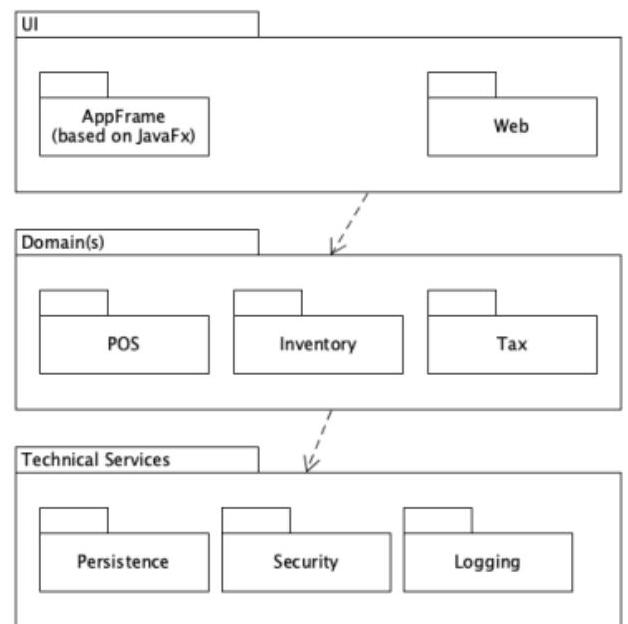
\includegraphics[width=0.9\linewidth]{images/2024_12_29_0d1d7b5551ea1b4b41bdg-09(1)}
\end{definition}

\begin{KR}{UML Diagrammauswahl}\\
Entscheidungshilfe für die Wahl des UML-Diagrammtyps:

\textbf{1. Strukturbeschreibung benötigt:}
\begin{itemize}
    \item Klassendiagramm für Typen und Beziehungen
    \item Paketdiagramm für Modularisierung
    \item Komponentendiagramm für Bausteinsicht
    \item Verteilungsdiagramm für Deployment
\end{itemize}

\textbf{2. Verhaltensbeschreibung benötigt:}
\begin{itemize}
    \item Sequenzdiagramm für Interaktionsabläufe
    \item Aktivitätsdiagramm für Workflows
    \item Zustandsdiagramm für Objektlebenszyklen
    \item Kommunikationsdiagramm für Objektkollaborationen
\end{itemize}

\textbf{3. Abstraktionsebene wählen:}
\begin{itemize}
    \item Analyse: Konzeptuelle Diagramme
    \item Design: Detaillierte Spezifikation
    \item Implementation: Codenahes Design
\end{itemize}
\end{KR}

\begin{concept}{Responsibility Driven Design (RDD)}\\
Design basierend auf Verantwortlichkeiten:
\begin{itemize}
    \item Klassenentwurf nach Rollen
    \item Kollaborationsbeziehungen
    \item Implementierung durch Attribute/Methoden
    \item Anwendbar auf allen Ebenen
\end{itemize}
\end{concept}

\begin{example2}{Prüfungsaufgabe: UML-Modellierung}
\textbf{Aufgabe:} 
Modellieren Sie für ein Bibliothekssystem die Ausleihe eines Buches mit:
\begin{itemize}
    \item Klassendiagramm der beteiligten Klassen
    \item Sequenzdiagramm des Ausleihvorgangs
    \item Zustandsdiagramm für ein Buchexemplar
\end{itemize}

\textbf{Bewertungskriterien:}
\begin{itemize}
    \item Korrekte UML-Notation
    \item Vollständigkeit der Modellierung
    \item Konsistenz zwischen Diagrammen
    \item Angemessener Detaillierungsgrad
\end{itemize}
%todo: add uml diagram
\end{example2}

\begin{theorem}{GRASP Prinzipien}\\
General Responsibility Assignment Software Patterns:
\begin{itemize}
    \item \textbf{Information Expert:} Verantwortung basierend auf Information
    \item \textbf{Creator:} Objekterstellung bei starker Beziehung
    \item \textbf{Controller:} Zentrale Steuerungslogik
    \item \textbf{Low Coupling:} Minimale Abhängigkeiten
    \item \textbf{High Cohesion:} Starker innerer Zusammenhang
    \item \textbf{Polymorphism:} Flexibilität durch Schnittstellen
    \item \textbf{Pure Fabrication:} Künstliche Klassen für besseres Design
    \item \textbf{Indirection:} Vermittler für Flexibilität
    \item \textbf{Protected Variations:} Kapselung von Änderungen
\end{itemize}
\end{theorem}

\begin{example2}{GRASP Anwendung}\\
\textbf{Szenario:} Online-Shop Warenkorb-Funktionalität

\textbf{GRASP-Prinzipien angewandt:}
\begin{itemize}
    \item \textbf{Information Expert:}
    \begin{itemize}
        \item Warenkorb kennt seine Positionen
        \item Berechnet selbst Gesamtsumme
    \end{itemize}
    
    \item \textbf{Creator:}
    \begin{itemize}
        \item Warenkorb erstellt Warenkorbpositionen
        \item Bestellung erstellt aus Warenkorb
    \end{itemize}
    
    \item \textbf{Controller:}
    \begin{itemize}
        \item ShoppingController koordiniert UI und Domain
        \item Keine Geschäftslogik im Controller
    \end{itemize}
    
    \item \textbf{Low Coupling:}
    \begin{itemize}
        \item UI kennt nur Controller
        \item Domain unabhängig von UI
    \end{itemize}
\end{itemize}
\end{example2}

\subsection{UML-Modellierung}

\begin{concept}{UML Diagrammtypen Übersicht}\\
UML bietet verschiedene Diagrammtypen für statische und dynamische Modellierung:

\textbf{Statische Modelle:}
\begin{itemize}
    \item Klassendiagramm
    \item Paketdiagramm
    \item Komponentendiagramm
    \item Verteilungsdiagramm
\end{itemize}

\textbf{Dynamische Modelle:}
\begin{itemize}
    \item Sequenzdiagramm
    \item Kommunikationsdiagramm
    \item Zustandsdiagramm
    \item Aktivitätsdiagramm
\end{itemize}
\end{concept}

\begin{definition}{Klassendiagramm}\\
\textbf{Hauptelemente:}
\begin{itemize}
    \item \textbf{Klassen:}
    \begin{itemize}
        \item Name der Klasse
        \item Attribute mit Sichtbarkeit
        \item Operationen mit Parametern
    \end{itemize}
    
    \item \textbf{Beziehungen:}
    \begin{itemize}
        \item Assoziation (normaler Pfeil)
        \item Vererbung (geschlossener Pfeil)
        \item Implementierung (gestrichelter Pfeil)
        \item Aggregation (leere Raute)
        \item Komposition (gefüllte Raute)
    \end{itemize}
    
    \item \textbf{Interfaces:}
    \begin{itemize}
        \item Stereotyp <<interface>>
        \item Nur Methodensignaturen
        \item Implementierungsbeziehung
    \end{itemize}
\end{itemize}
\end{definition}

\begin{example2}{Klassendiagramm: E-Commerce System}\\
\textbf{Domänenmodell mit wichtigen Beziehungen:}

\begin{lstlisting}[language=Java, style=basesmol]
public interface OrderRepository {
    Optional<Order> findById(OrderId id);
    void save(Order order);
}

public class Order {
    private OrderId id;
    private Customer customer;
    private List<OrderLine> orderLines;
    private OrderStatus status;
    
    public Money calculateTotal() {
        return orderLines.stream()
                        .map(OrderLine::getSubTotal)
                        .reduce(Money.ZERO, Money::add);
    }
}

public class OrderLine {
    private Product product;
    private int quantity;
    private Money price;
    
    public Money getSubTotal() {
        return price.multiply(quantity);
    }
}
\end{lstlisting}
\end{example2}

\begin{definition}{Sequenzdiagramm}\\
\textbf{Notationselemente:}
\begin{itemize}
    \item \textbf{Lebenslinien:}
    \begin{itemize}
        \item Objekte als Rechtecke
        \item Vertikale gestrichelte Linie
        \item Aktivierungsbalken für Ausführung
    \end{itemize}
    
    \item \textbf{Nachrichten:}
    \begin{itemize}
        \item Synchron (durchgezogener Pfeil)
        \item Asynchron (offener Pfeil)
        \item Antwort (gestrichelter Pfeil)
        \item Parameter und Rückgabewerte
    \end{itemize}
    
    \item \textbf{Kontrollelemente:}
    \begin{itemize}
        \item alt (Alternative)
        \item loop (Schleife)
        \item opt (Optional)
        \item par (Parallel)
    \end{itemize}
\end{itemize}
\end{definition}

\begin{example2}{Sequenzdiagramm: Bestellprozess}\\
\textbf{Interaktion zwischen Komponenten:}

\begin{lstlisting}[language=Java, style=basesmol]
public class OrderService {
    private final OrderRepository orderRepo;
    private final PaymentService paymentService;
    
    public OrderConfirmation processOrder(OrderRequest request) {
        // Validiere Bestellung
        validateOrder(request);
        
        // Erstelle Order
        Order order = createOrder(request);
        orderRepo.save(order);
        
        // Prozessiere Zahlung
        PaymentResult result = paymentService
            .processPayment(order.getId(), order.getTotal());
            
        // Bestaetige Bestellung
        if (result.isSuccessful()) {
            order.confirm();
            orderRepo.save(order);
            return new OrderConfirmation(order);
        }
        
        throw new PaymentFailedException();
    }
}
\end{lstlisting}
\end{example2}

\begin{definition}{Zustandsdiagramm}\\
\textbf{Notationselemente:}
\begin{itemize}
    \item \textbf{Zustände:}
    \begin{itemize}
        \item Startzustand (gefüllter Kreis)
        \item Endzustand (Kreis mit Punkt)
        \item Einfache Zustände (Rechteck)
        \item Zusammengesetzte Zustände
    \end{itemize}
    
    \item \textbf{Transitionen:}
    \begin{itemize}
        \item Event [Guard] / Action
        \item Interne Transitionen
        \item Selbsttransitionen
    \end{itemize}
    
    \item \textbf{Spezielle Elemente:}
    \begin{itemize}
        \item History State (H)
        \item Deep History (H*)
        \item Entry/Exit Points
        \item Choice Points
    \end{itemize}
\end{itemize}
\end{definition}

\begin{example2}{Zustandsdiagramm: Bestellstatus}\\
\textbf{Implementation eines State Patterns:}

\begin{lstlisting}[language=Java, style=basesmol]
public interface OrderState {
    void process(Order order);
    void cancel(Order order);
    void ship(Order order);
}

public class NewOrderState implements OrderState {
    @Override
    public void process(Order order) {
        validateOrder(order);
        order.setState(new ProcessingState());
    }
    
    @Override
    public void cancel(Order order) {
        order.setState(new CancelledState());
    }
    
    @Override
    public void ship(Order order) {
        throw new IllegalStateException(
            "Cannot ship new order");
    }
}

public class Order {
    private OrderState state;
    
    public void process() {
        state.process(this);
    }
    
    void setState(OrderState newState) {
        this.state = newState;
    }
}
\end{lstlisting}
\end{example2}

\begin{definition}{Aktivitätsdiagramm}\\
\textbf{Hauptelemente:}
\begin{itemize}
    \item \textbf{Aktionen:}
    \begin{itemize}
        \item Atomare Aktionen
        \item Call Behavior Action
        \item Send/Receive Signal
    \end{itemize}
    
    \item \textbf{Kontrollfluss:}
    \begin{itemize}
        \item Verzweigungen (Diamond)
        \item Parallelisierung (Balken)
        \item Join/Merge Nodes
    \end{itemize}
    
    \item \textbf{Strukturierung:}
    \begin{itemize}
        \item Activity Partitions (Swimlanes)
        \item Structured Activity Nodes
        \item Interruptible Regions
    \end{itemize}
\end{itemize}
\end{definition}

\begin{example2}{Aktivitätsdiagramm: Bestellabwicklung}\\
\textbf{Implementation eines Geschäftsprozesses:}

\begin{lstlisting}[language=Java, style=basesmol]
public class OrderProcessor {
    public void processOrder(Order order) {
        // Parallele Verarbeitung
        CompletableFuture.allOf(
            validateInventory(order),
            validatePayment(order)
        ).thenRun(() -> {
            if (order.isValid()) {
                fulfillOrder(order);
            } else {
                handleValidationFailure(order);
            }
        });
    }
    
    private CompletableFuture<Void> validateInventory(
            Order order) {
        return CompletableFuture.runAsync(() -> {
            order.getItems().forEach(item -> {
                if (!inventoryService.isAvailable(item)) {
                    throw new OutOfStockException(item);
                }
            });
        });
    }
}
\end{lstlisting}
\end{example2}

\begin{definition}{Verteilungsdiagramm}\\
\textbf{Elemente:}
\begin{itemize}
    \item \textbf{Nodes:}
    \begin{itemize}
        \item Device Nodes
        \item Execution Environment
        \item Artifacts
    \end{itemize}
    
    \item \textbf{Verbindungen:}
    \begin{itemize}
        \item Kommunikationspfade
        \item Protokolle
        \item Multiplizitäten
    \end{itemize}
    
    \item \textbf{Deployment:}
    \begin{itemize}
        \item Deployment Specifications
        \item Manifestationen
    \end{itemize}
\end{itemize}
\end{definition}

\begin{example2}{Verteilungsdiagramm: Microservice-Architektur}\\
\textbf{Deployment-Konfiguration:}

\begin{lstlisting}[language=Java, style=basesmol]
@Configuration
public class ServiceConfig {
    @Value("${service.host}")
    private String serviceHost;
    
    @Value("${service.port}")
    private int servicePort;
    
    @Bean
    public ServiceRegistry registry() {
        return ServiceRegistry.builder()
            .host(serviceHost)
            .port(servicePort)
            .healthCheck("/health")
            .build();
    }
    
    @Bean
    public LoadBalancer loadBalancer(
            ServiceRegistry registry) {
        return new RoundRobinLoadBalancer(registry);
    }
}
\end{lstlisting}
\end{example2}

\begin{definition}{Kommunikationsdiagramm}\\
\textbf{Hauptelemente:}
\begin{itemize}
    \item \textbf{Objekte:}
    \begin{itemize}
        \item Als Rechtecke dargestellt
        \item Mit Objektname und Klasse
        \item Verbunden durch Links
    \end{itemize}
    
    \item \textbf{Nachrichten:}
    \begin{itemize}
        \item Nummerierte Sequenz
        \item Synchrone/Asynchrone Aufrufe
        \item Parameter und Rückgabewerte
    \end{itemize}
    
    \item \textbf{Steuerungselemente:}
    \begin{itemize}
        \item Bedingte Nachrichten [condition]
        \item Iterationen *
        \item Parallele Ausführung || 
    \end{itemize}
\end{itemize}
\end{definition}

\begin{example2}{Kommunikationsdiagramm: Shopping Cart}\\
\textbf{Objektinteraktionen beim Checkout:}

\begin{lstlisting}[language=Java, style=basesmol]
public class ShoppingCart {
    private List<CartItem> items;
    private CheckoutService checkoutService;
    
    public Order checkout() {
        // 1: validateItems()
        validateItems();
        
        // 2: calculateTotal()
        Money total = calculateTotal();
        
        // 3: createOrder(items, total)
        Order order = checkoutService.createOrder(
            items, total);
            
        // 4: clearCart()
        items.clear();
        
        return order;
    }
}
\end{lstlisting}
\end{example2}

\begin{definition}{Paketdiagramm}\\
\textbf{Elemente:}
\begin{itemize}
    \item \textbf{Pakete:}
    \begin{itemize}
        \item Gruppierung von Modellelementen
        \item Hierarchische Strukturierung
        \item Namensräume
    \end{itemize}
    
    \item \textbf{Abhängigkeiten:}
    \begin{itemize}
        \item Import/Export von Elementen
        \item <<use>> Beziehungen
        \item Zugriffsrechte
    \end{itemize}
\end{itemize}
\end{definition}

\begin{KR}{UML Diagrammauswahl}\\
Entscheidungshilfen für die Wahl des passenden Diagrammtyps:

\textbf{1. Statische Struktur}
\begin{itemize}
    \item Klassendiagramm für Typen und Beziehungen
    \item Paketdiagramm für Modularisierung
    \item Komponentendiagramm für Bausteinsicht
    \item Verteilungsdiagramm für physische Verteilung
\end{itemize}

\textbf{2. Dynamisches Verhalten}
\begin{itemize}
    \item Sequenzdiagramm für zeitliche Abläufe
    \item Kommunikationsdiagramm für Objektkollaborationen
    \item Zustandsdiagramm für Objektlebenszyklen
    \item Aktivitätsdiagramm für Geschäftsprozesse
\end{itemize}

\textbf{3. Verwendungszweck}
\begin{itemize}
    \item Analyse: Konzeptuelle Modellierung
    \item Design: Detaillierte Spezifikation
    \item Implementation: Code-nahe Darstellung
    \item Dokumentation: Architekturübersicht
\end{itemize}
\end{KR}

\begin{example2}{UML in der Praxis}\\
\textbf{Beispiel eines kompletten Designs:}

\begin{lstlisting}[language=Java, style=basesmol]
// Paketstruktur
package com.example.shop;

// Domain Model
public class Product {
    private ProductId id;
    private String name;
    private Money price;
    private Category category;
}

// Service Layer
@Service
public class ProductService {
    private final ProductRepository repository;
    private final PriceCalculator calculator;
    
    public Product updatePrice(
            ProductId id, Money newPrice) {
        Product product = repository.findById(id)
            .orElseThrow(ProductNotFoundException::new);
            
        Money calculatedPrice = calculator
            .calculateFinalPrice(newPrice);
            
        product.updatePrice(calculatedPrice);
        return repository.save(product);
    }
}

// Controller Layer
@RestController
@RequestMapping("/api/products")
public class ProductController {
    private final ProductService service;
    
    @PutMapping("/{id}/price")
    public ProductDTO updatePrice(
            @PathVariable ProductId id,
            @RequestBody PriceUpdateRequest request) {
        Product product = service.updatePrice(
            id, request.getNewPrice());
        return ProductDTO.from(product);
    }
}
\end{lstlisting}
\end{example2}

\pagebreak



\subsection{other examples}

\begin{example2}{Gute Testbarkeit}\\

\begin{lstlisting}[language=Java, style=basesmol]
public class OrderService {
    private final OrderRepository repository;
    private final PaymentGateway paymentGateway;
    
    // Dependency Injection ermoeglicht einfaches Mocking
    public OrderService(
            OrderRepository repository,
            PaymentGateway paymentGateway) {
        this.repository = repository;
        this.paymentGateway = paymentGateway;
    }
    
    // Klare Methoden-Verantwortlichkeiten
    public OrderResult createOrder(OrderRequest request) {
        validateRequest(request);
        Order order = createOrderEntity(request);
        PaymentResult payment = processPayment(order);
        return createOrderResult(order, payment);
    }
}
\end{lstlisting}
\end{example2}

\subsubsection{Dokumentation Architektur}

\begin{example2}{Architekturanalyse}\\
\textbf{Analyse für ein E-Commerce-System:}

\begin{lstlisting}[language=Java, style=basesmol]
// Dokumentation der Analyse
public class ArchitectureAnalysis {
    public class QualityRequirement {
        String name;
        String description;
        int priority;
        String measurementCriteria;
    }
    
    public class ArchitecturalConstraint {
        String type; // Technical, Organizational, Business
        String description;
        String impact;
    }
    
    // Beispiel Qualitaetsanforderung
    QualityRequirement performance = new QualityRequirement(
        "Response Time",
        "System responses within 200ms",
        1,
        "95th percentile < 200ms"
    );
    
    // Beispiel Randbedingung
    ArchitecturalConstraint technology = new ArchitecturalConstraint(
        "Technical",
        "Must use Java 17",
        "Affects framework selection"
    );
}
\end{lstlisting}
\end{example2}

\begin{example2}{Architektur-Entscheidungen}\\
\textbf{Entscheidungsdokumentation:}

\begin{lstlisting}[language=Java, style=basesmol]
public class ArchitectureDecision {
    String id;
    String title;
    String context;
    String decision;
    String rationale;
    List<String> consequences;
    List<Alternative> alternatives;
    
    class Alternative {
        String description;
        List<String> pros;
        List<String> cons;
        String rejectionReason;
    }
}

// Beispiel:
ArchitectureDecision caching = new ArchitectureDecision(
    "AD001",
    "Caching Strategy",
    "High read load on product catalog",
    "Use Redis as distributed cache",
    "Better performance and scalability",
    List.of("Requires Redis expertise", 
            "Additional infrastructure"),
    List.of(new Alternative(
        "In-memory cache",
        List.of("Simple", "No additional infrastructure"),
        List.of("Not distributed", "Memory limited"),
        "Doesn't scale horizontally"
    ))
);
\end{lstlisting}
\end{example2}

\begin{example2}{Architektur-Review}\\
\textbf{Review-Protokoll:}

\begin{lstlisting}[language=Java, style=basesmol]
public class ArchitectureReview {
    public class Finding {
        String area;
        String observation;
        Risk risk;
        String recommendation;
        Priority priority;
    }
    
    public class Action {
        String description;
        String responsible;
        LocalDate dueDate;
        Status status;
    }
    
    List<Finding> findings = List.of(
        new Finding(
            "Security",
            "Missing rate limiting",
            Risk.HIGH,
            "Implement API gateway with rate limiting",
            Priority.HIGH
        )
    );
    
    List<Action> actions = List.of(
        new Action(
            "Implement API gateway",
            "Team A",
            LocalDate.now().plusWeeks(2),
            Status.OPEN
        )
    );
}
\end{lstlisting}
\end{example2}

\subsection{Praktische Anwendung}

\begin{KR}{Architektur-Dokumentation}
\textbf{1. Überblick}
\begin{itemize}
    \item Systemkontext
    \item Hauptkomponenten
    \item Technologie-Stack
\end{itemize}

\textbf{2. Architektur-Entscheidungen}
\begin{itemize}
    \item Begründungen
    \item Alternativen
    \item Trade-offs
\end{itemize}

\textbf{3. Technische Konzepte}
\begin{itemize}
    \item Persistenz
    \item Sicherheit
    \item Integration
    \item Deployment
\end{itemize}

\textbf{4. Qualitätsszenarien}
\begin{itemize}
    \item Performance
    \item Skalierbarkeit
    \item Verfügbarkeit
    \item Wartbarkeit
\end{itemize}
\end{KR}

\begin{example2}{Architektur-Dokumentation: REST API}
\begin{lstlisting}[language=Java, style=basesmol]
@RestController
@RequestMapping("/api/v1/orders")
public class OrderController {
    
    @GetMapping("/{id}")
    @Operation(summary = "Get order by ID",
              description = "Returns detailed order information")
    @ApiResponses({
        @ApiResponse(responseCode = "200", 
                    description = "Order found"),
        @ApiResponse(responseCode = "404", 
                    description = "Order not found")
    })
    public OrderDTO getOrder(@PathVariable String id) {
        return orderService.findById(id)
                          .map(OrderDTO::from)
                          .orElseThrow(OrderNotFoundException::new);
    }
}
\end{lstlisting}

\textbf{Qualitätsszenarien:}
\begin{itemize}
    \item Response Time < 200ms (95. Perzentil)
    \item Verfügbarkeit 99.9%
    \item Maximal 1000 req/s pro Instance
    \item Automatische Skalierung ab 70% CPU
\end{itemize}
\end{example2}

\begin{KR}{Architektur-Review}
\textbf{1. Vorbereitung}
\begin{itemize}
    \item Review-Team zusammenstellen
    \item Dokumentation aufbereiten
    \item Checklisten erstellen
    \item Zeitplan festlegen
\end{itemize}

\textbf{2. Durchführung}
\begin{itemize}
    \item Architektur vorstellen
    \item Szenarien durchspielen
    \item Qualitätsattribute prüfen
    \item Risiken identifizieren
\end{itemize}

\textbf{3. Nachbereitung}
\begin{itemize}
    \item Findings dokumentieren
    \item Maßnahmen definieren
    \item Priorisierung vornehmen
    \item Follow-up planen
\end{itemize}
\end{KR}

\begin{example2}{Typische Design-Aufgaben}
\textbf{1. REST API Design}
\begin{lstlisting}[language=Java, style=basesmol]
// API Definition
@RestController
@RequestMapping("/api/v1/products")
public class ProductController {
    private final ProductService service;
    
    @GetMapping
    public PagedResponse<ProductDTO> getProducts(
            @RequestParam(defaultValue = "0") int page,
            @RequestParam(defaultValue = "20") int size) {
        return service.findAll(page, size);
    }
    
    @PostMapping
    @ResponseStatus(HttpStatus.CREATED)
    public ProductDTO createProduct(
            @RequestBody @Valid CreateProductRequest request) {
        return service.createProduct(request);
    }
}

// Service Layer
@Service
public class ProductService {
    private final ProductRepository repository;
    private final ProductValidator validator;
    
    public ProductDTO createProduct(CreateProductRequest request) {
        validator.validate(request);
        Product product = new Product(request);
        repository.save(product);
        return ProductDTO.from(product);
    }
}

// Domain Layer
@Entity
public class Product {
    @Id
    private String id;
    private String name;
    private Money price;
    private ProductStatus status;
    
    public void updatePrice(Money newPrice) {
        validatePrice(newPrice);
        this.price = newPrice;
    }
}
\end{lstlisting}
\end{example2}

\begin{KR}{Typische Implementierungsmuster}
\textbf{1. Schichtenarchitektur}
\begin{itemize}
    \item Controller für API
    \item Service für Geschäftslogik
    \item Repository für Persistenz
    \item Entities für Domänenmodell
\end{itemize}

\textbf{2. Cross-Cutting Concerns}
\begin{itemize}
    \item Exception Handling
    \item Validierung
    \item Logging
    \item Security
\end{itemize}

\textbf{3. Testing}
\begin{itemize}
    \item Unit Tests
    \item Integration Tests
    \item End-to-End Tests
    \item Performance Tests
\end{itemize}
\end{KR}

\begin{example2}{Implementierung einer Microservice-Architektur}
\begin{lstlisting}[language=Java, style=basesmol]
// Service Discovery
@SpringBootApplication
@EnableEurekaServer
public class ServiceRegistryApplication {
    public static void main(String[] args) {
        SpringApplication.run(
            ServiceRegistryApplication.class, args);
    }
}

// API Gateway
@Configuration
public class GatewayConfig {
    @Bean
    public RouteLocator customRouteLocator(
            RouteLocatorBuilder builder) {
        return builder.routes()
            .route("product_route", r -> r
                .path("/products/**")
                .filters(f -> f
                    .circuitBreaker(c -> c
                        .setName("productCB")
                        .setFallbackUri("forward:/fallback"))
                    .retry(3))
                .uri("lb://product-service"))
            .build();
    }
}

// Circuit Breaker
@Service
public class ProductService {
    @CircuitBreaker(name = "productService",
                   fallbackMethod = "getProductFallback")
    public Product getProduct(String id) {
        return productClient.getProduct(id);
    }
    
    public Product getProductFallback(String id,
            Exception ex) {
        return getCachedProduct(id);
    }
}
\end{lstlisting}
\end{example2}